% VARIABLES %%%
\def\theme{Devoir sur temps libre 3}
\def\date{20/01/2024}
%%%%%%%%%%%%%%%

% DEFINITIONS %
\newcommand{\grandeurs}[1]{
    Grandeurs mise en jeu:
    \begin{itemize}
        #1
    \end{itemize}
}
\def\emm{\ensuremath{\euro\slash\meter^{2}}}

\newcommand{\rEnum}[1]{
    \begin{enumerate}[label=\textbf{\color{red}\roman*.}]
        #1
    \end{enumerate}
}
\newcommand{\aEnum}[1]{
    \begin{enumerate}[label=\textbf{\color{red}\alph*.}]
        #1
    \end{enumerate}
}
\newcommand{\nEnum}[1]{
    \begin{enumerate}[label=\textbf{\arabic*.}]
        #1
    \end{enumerate}
}
\newcommand{\sItem}[1]{
    \begin{itemize}[wide, labelwidth=!, labelindent=0pt]
        #1
    \end{itemize}
}
\newcommand{\file}[1]{%
    {\fontfamily{qhv}\selectfont % phv is Helvetica
    \textit{\color{Fuchsia}$\hookrightarrow$ \small Pesin\_partie#1}}%
}

\def\OU{\color{red}OU \color{black}}
\def\ET{\color{blue}ET \color{black}}

\def\tikzScale{0.9cm}
\def\gridWidth{0.1mm}
\def\gridSize{5}

\newcommand{\drawNum}[3]{
    \def\numColor{black}
    \ifthenelse{\equal{#1}{1}}{\def\numColor{red}}{}
    \node[shift={(-0.5,-0.5)}, color = \numColor] at (#2,#3) {#1};
}
\newcommand{\eraseNum}[3]{
    \def\numColor{white}
    \node[shift={(-0.5,-0.5)}, color = \numColor] at (#2,#3) {#1};
}

\newcommand{\drawDay}[1]{
    \drawGrid{\gridSize}{\gridSize}{\gridWidth};
    \foreach \n in {1,...,\gridSize}
        \foreach \m in {1,...,\gridSize}
            \drawNum{0}{\m}{\n};
    \node at (2.5,-0.5) {jour #1};
}

\newcommand{\spread}[2]{
    \eraseNum{0}{#1}{#2}
    \drawNum{1}{#1}{#2};
}

\newcommand{\python}[1]{\lstinputlisting[language=Python]{resources/dm3/#1}}

%%%%%%%%%%%%%%

\section*{Partie A – Solides, volumes et contenances – Cycle 4}
\aEnum{
    \item \grandeurs{
        \item \textbf{Volume} d'eau : grandeur principale à estimer.
        \item \textbf{Hauteur} d'eau dans la bouteille.
        \item \textbf{Hauteur} et \textbf{diamètre} de la bouteille.
        \item \textbf{Périmètres} et \textbf{aires} pour différentes sections de la bouteille.
    }

    \item 
    \nEnum{
        \item\;
        \begin{enumerate}[label= Modélisation \arabic* $\rightarrow$]
            \item Figure 4 (cylindre simple avec la hauteur d'eau représentée)
            \item Figure 2 (cylindre surmonté d'un cône)
            \item Figure 8 (parallélépipède rectangle de hauteur inférieure à sa largeur)
            \item Figures 1 et 6 (cylindre et rayon égale à la largeur de la bouteille)
            \item Figures 1 et 5 (cylindre et rayon égale à la «diagonale» de la vue de dessus)
            \item Figures 3 et 7 (parallélépipède rectangle de base carrée)
        \end{enumerate}
        \item Chacune des modélisations apporte de bonnes idée, cependant certaines semble plus pertinentes que d'autres. 
        \begin{itemize}[wide, labelwidth=!, labelindent=0pt]
            \item D'une part les modélisation 4 et 2 se base sur une estimation, qui n'apparaît pas dans l'énoncé,
            du volume total de la bouteille, et s'en sert pour trouver le rayon.
            Entre les deux,
            le modèle 2 semble être le plus pertinent;
            car il prend en compte le changement de profil au niveau du goulot.
            \item Pour cette même question de profil on peut rejeter la modélisation 6;
            car couché,
            le niveau d'eau sera davantage influencé par l'allure du goulot.
            \item Ainsi les modélisations 3, 4 et 5 semble être les plus pertinentes;
            car elle s'appuie sur les données de l'énoncé et n'on pas à considérer la forme du haut de la bouteille.
            Parmi ces 3 modélisations, on voit sur les figures 5, 6 et 7,
            que le choix d'une base carrée semble être le plus éloigné de la réalité,
            et ainsi,
            le modèle 3 semble être le moins pertinent des 3.
        \end{itemize}
    }

    \item \file{A.ggb} \rEnum{
        \item Dans le graphe 3D à côté de la modélisation de la bouteille.
        \item J'ai choisi de convertir les donnés en décimètres afin d'obtenir naturellement une réponse en litres.
        \item 
        \begin{itemize}[wide, labelwidth=!, labelindent=0pt] 
            \item Je n'ai pas réalisé un prisme de base carré au bord arrondi comme la bouteille l'est dans la réalité,
            mais j'ai approché cette forme par un octogon obtenu en tracant 4 tangante repartie régulièrement au cercle de la modélisation 4,
            et en prenant ensuite comme point de ma base les intersections avec le cercle de la modélisation 5.
            \item Je n'ai également pas modélisé le changement de section de la bouteille au niveau de sa base ou par les stries qui marque la bouteille car cela semble être une tache difficile avec peu de conséquences.
            \item J'ai aussi mis de côté le problème du renfoncement qu'il existe au fond de la bouteille encore une fois sans grandes conséquences.
        \end{itemize}
    }
}

\newpage
\section*{Partie B – Construction de boîtes – Cycle 4 - lycée}

\begin{enumerate}[label=\textbf{\color{red}\arabic*. \color{black}situation \arabic*}, wide, labelwidth=!, labelindent=0pt]
    \item
    \aEnum{
        \item \grandeurs{
            \item \textbf{Volume} de la boite.
            \item \textbf{Longueur} et \textbf{largeur} de la feuille.
            \item \textbf{Longueur} du côté du carré.
            \item \textbf{Longueur}, \textbf{largeur} et \textbf{hauteur} de la boite.
        }
        \item \file{B-1b.ods} La feuille de calcul proposé,
        permet de determiner le volume de la boite de papier lorsque l'on modifie dans la colonne F la valeur du côté du carré.
        On peut alors chercher la valeur optimal par balayage.
        \item \file{B-1c.ggb} Dans le fichier on retrouve un curseur qui nous permet de modifier la mesure du côté du carré,
        et qui modifie dynamiquement le patron nécessaire à la création de la boite correspondant.
        On a ajouté sur la figure deux segments ainsi que leurs mesures,
        qui montre bien que la taille de la feuille dans laquelle on a coupé nos carrés reste inchangée.
        \item \rEnum{
            \item \file{B-1d-1.ggb} On peut enregistrer la valeur du côté du carré ainsi que celle du volume de la boite dans le tableur de géogebra,
            puis en bougeant le curseur balayer les valeurs à la main.
            \item \file{B-1d-2.ggb} En seconde on peut introduire une fonction qui donne le volume en fonction du côté du carré,
            puis trouver une valeur approché de l'extremum grace à l'outil points spéciaux.
            \item \file{B-1d-3.py}
        }
        \item Non car l'algorithme de dichotomie permet de trouver les racines d'une fonctions.
        On pourrait cependant l'appliquer à la dérivée et aisin trouver le maximum.
        \item Soient $l = 22\cm$ la longueur de la feuille et $L = 18\cm$ sa largeur,
        et $f$ la fonction qui donne le volume de la boite en fonction du côté du carré.\\
        On a pour $x\in[0;9]$: 
        \begin{align*}
            f(x) &= x \times (l - 2x) \times (L-2x)\\
            &= 4 x^3 - 2 (l+L) x + lL\\
            \shortintertext{et $f$ est dérivable sur [0;9] alors}
            f'(x) &= 12 x^2 - 4(l+L) x + lL\\
            \shortintertext{on peut trouver ces racines avec le discriminant}
            \Delta &= (-4(l+L))^2 - 4 \times 12 + lL
            = 6592
            \shortintertext{on trouve alors les racines}
            x_1 &= \frac{4(l+L) + sqrt(\Delta)}{2 \times 12}
            = \frac{20 + \sqrt{103}}{3} > 9 \textrm{ hors de l'interval}
            \iet x_2 &= \frac{20 - \sqrt{103}}{3} \approx 3,2837
            \iet f(x_2) &\approx 579,36
        \end{align*} 
        On trouve alors un maximum pour $x_2 = \frac{20 - \sqrt{103}}{3}$.
        Un carré de côté $x_2$ produirait donc la boite de volume maximal.
        \item Si on prend une feuille de dimension $15\cm \times 24\cm$,
        alors la solution est un carré de côté $3\cm$.
    }

    \item
    \aEnum{
        \item \grandeurs{
            \item \textbf{Volume} de la boite.
            \item \textbf{Longueur} et \textbf{largeur} de la feuille de carton.
            \item \textbf{Longueur} du côté du carré.
            \item \textbf{Longueur}, \textbf{largeur} et \textbf{hauteur} de la boite.
        }
        \item Soient $l = 45\cm$ la longueur de la feuille et $L = 30\cm$ sa largeur,
        et $f$ la fonction qui donne le volume de la boite en fonction du côté du carré.\\
        On a pour $x\in[0;10]$:
        \begin{align*}
            f(x) &= x \times \frac{(l - 3x)}{2} \times (L-2x)\\
            &= x \times \frac{45-3x}{2} \times (30 - 2x)
            \ialors f'(x) &= 9 \times x^2- 180 x + 675
            \ialors \Delta &= 8100
            \ialors x_1 &=15 > 10
            \iet x_2 &= 5
            \iet f(x_2) &= 1500
        \end{align*}
        On trouve donc une boite de dimension $\frac{(l - 3x_2)}{2} \times (L-2x_2) \times x$,
        c'est a dire:\\
        $15\cm \times 20\cm \times 5\cm$
        \item Le résultat étant entier les méthodes d'approximations perdent de leur interet.
        Chercher à augmenter la précision du résultat (les décimales corrects) semblera un peu artificiel.
        \item Un élève de cycle 4 pourra trouver le résultat par essaie erreur car il est entier.
        Cela-dit il sera incapable de justifier le fait qu'il sagit réellement de la réponse n'ayant pas connaissance sur la dérivation,
        qui lui permettrais de vérifier qu'il sagit bien d'un extremum.
    }

    \item
    \aEnum{
        \item \grandeurs{
            \item \textbf{Volume} du garage ($\meter^3$).
            \item \textbf{Profondeur}, \textbf{largeur} et \textbf{hauteur} du garage (\meter).
            \item \textbf{Surface} en bois de la porte et \textbf{surface} en tôle de la paroi ($\meter^2$)
            \item \textbf{Rapport Prix / Surface} de la tôle et du bois (\emm)
            \item \textbf{Prix} de la tôle et du bois (\euro)
        }
        \item Le choix de noter $x$ la largeur est $h$ la hauteur n'est pas anodin dans ce schéma.
        En effet on peut vite se rendre compte que la profondeur et le volume étant fixé,
        déterminer l'une des deux grandeurs fixé plus tot fixera la seconde.
        Et nommer ainsi un élève aura naturellement envie de faire varier la largeur et non pas la hauteur,
        car on à l'habitude de nommer nos variables $x$ dans l'étude de fonctions.
        \item \file{B-3.ggb}
        \rEnum{
            \item Avant de réaliser le fichier il faut se demander qu'elle valeur sera notre variable principale,
            et comment elle déterminera le reste de nos valeurs.
            On a:
            \begin{align*}
                \textrm{largeur} \times \textrm{profondeur} \times \textrm{hauteur} &= \textrm{volume}\\
                x \times 6 \times h &= 75
                \ialors x \times h &= \frac{75}{6}
            \end{align*}
            On peut donc choisir soit $x$ soit $h$ comme variable, l'autre sera déterminer par ce choix.
            \item On choisi de manière naturel,
            comme évoqué en \color{red}\textbf{b.}\color{black},
            $x$ comme curseur.
            \item Pour trouver la solution optimal, le fichier comprend un graphique ou apparait un point $F($largeur$,$prix total$)$ avec sa trace,
            celà permet d'avoir une idée d'ou ce trouve le minimum en manipulant le curseur largeur.
            Puis pour affiner le resultat un tableur enregistre les valeurs largeur, hauteur et prix pour pouvoir répondre à la question.
        }
    }
\end{enumerate}

\section*{Partie C – Ouverture}

\begin{enumerate}[label=\textbf{\color{red}\arabic*.}]
    \item Ce modèle semble assé pertinent pour simuler un feu de forêt,
    même si on y a fait de grosse modélisation entrainent certains renoncements:
    \sItem{
        \item La forêt est supposé de densité régulière;
        ainsi le feu se propage suivant les même règles sur toutes les cases.
        \item Une case ne peu pas resté en feu pendant plus d'un tour et ainsi affecter d'autres cases.
        \item La forêt est forcément de forme rectangulaire et il ne peut pas y avoir de clairière.
    }
    \item \aEnum{
        \item \textit{(Je suppose que l'énoncé:
        «90\% de chance de contaminer un ou des individus avec qui il est en contact»
        repose sur le même principe que la forêt.)}\\
        J'utilise le générateur de nombre aléatoire de la calculatrice numworks,
        il donne un nombre dans $[0;1[$.
        \nEnum{
            \item Chaque jour je regarde (dans le sens de lecture français) chaques cases 1 avec au moins une case 0 dans ces voisins direct.
            \item Pour ces cases je regarde chacune des cases 0 voisines (en commencant par le nord puis dans le sens indirect) et je génère un nombre aléatoire.
            \item Si le nombre généré est supérieur à 0.1 je change le 0 en 1.
            \item Je passe au jour suivant.
        } 
    \begin{center}
        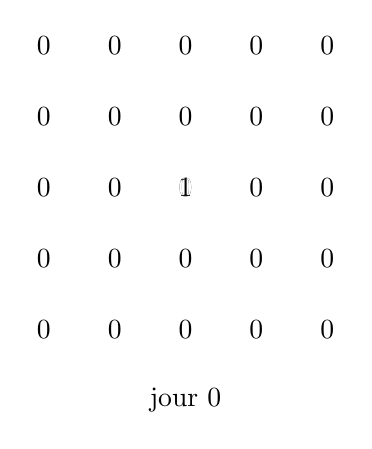
\begin{tikzpicture}[x=\tikzScale, y=\tikzScale]
            \drawDay{0};

            % init
            \spread{3}{3};

        \end{tikzpicture}
        \hfill
        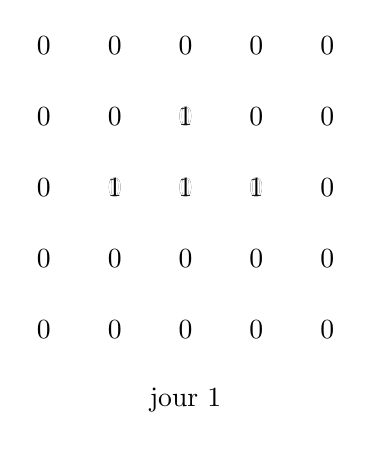
\begin{tikzpicture}[x=\tikzScale, y=\tikzScale]
            \drawDay{1};

            \spread{3}{3};

            % 3 3
            \spread{3}{4};
            \spread{4}{3};
            \spread{2}{3};

        \end{tikzpicture}
        \hfill
        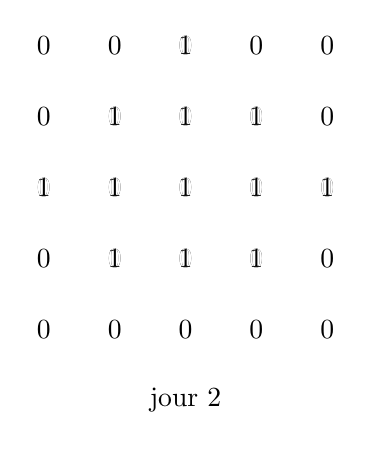
\begin{tikzpicture}[x=\tikzScale, y=\tikzScale]
            \drawDay{2};
            
            \spread{3}{3};
            
            \spread{3}{4};
            \spread{4}{3};
            \spread{2}{3};

            % 3 4
            \spread{4}{4};
            \spread{2}{4};
            \spread{3}{5};

            % 2 3
            \spread{2}{2};
            \spread{1}{3};

            % 3 3
            \spread{3}{2};

            % 4 3
            \spread{5}{3};
            \spread{4}{2};
        \end{tikzpicture}
    \end{center}
        \item \file{C-2.ods}\\
        Formule entrée dans la cellule C7:\\
        = SI(((ALEA() < \$C\$3) \ET (C6 = 1))\\
        \OU ((ALEA() < \$C\$3) \ET (D7 = 1))\\
        \OU ((ALEA() < \$C\$3) \ET (C8 = 1))\\
        \OU ((ALEA() < \$C\$3) \ET (B7 = 1));\\
        1; C7)
        \item Il faut environ 4 jours pour infecter tous le monde.
    }

    Être capable de calculer le coefficient multiplicateur pour un taux d'évolution donné
    Construire un modèle à partir de fréquences observées, en distinguant
    nettement modèle et réalité.
    \item \aEnum{
        \item \file{C-3.ods}
        \item Connaissance : \sItem{
            \item \textbf{Évolutions successives} : Être capable de calculer le coefficient multiplicateur pour un taux d'évolution donné
            \item \textbf{Loi (distribution) de probabilité} : Construire un modèle à partir de fréquences observées, en distinguant
            nettement modèle et réalité.
        }
        \item Pensez à bien prendre en compte les personnes immunisés dans vos calculs.
    }
    \item \file{C-4.py}
    \nEnum{
        \item \python{C-4-a.py}
        La matrice est mise sous forme de liste.
        Pour acceder à une valeur,
        il faut alors convertir son indice bidimensionnels $(a,b)$ en indice unidimensionnel,
        donné par l'opération:
        \begin{equation*}
            b \times x+a
        \end{equation*}

        \item \python{C-4-b-1.py}
        $i$ est un indice unidimensionnel,
        on peut trouver sur quelle colonne il se trouve en prenant son reste modulo $x$ le nombre de colonnes.\\
        La colonne $0$ correspondant à la colonne de gauche, on teste si on ne s'y trouve pas.\\
        Et si random() qui donne un nombre etre 0 et 1 est inférieure à p alors on contamine le voisins de gauche.
        L'indice unidimensionnel du voisins de gauche est donné par $i-1$.

        \item \python{C-4-b-2.py}
        Colonne de droite: $x-1$\\
        Indice unidimensionnel du voisins de droite: $i+1$.
    
        \item \python{C-4-b-3.py}
        Ligne donné par le quotient dans la division euclidienne par $x$ de $i$.\\
        Ligne du bas: $0$\\
        Indice unidimensionnel du voisins du bas: $i-x$.
    
        \item \python{C-4-b-4.py}
        Ligne du haut: $y-1$\\
        Indice unidimensionnel du voisins du haut: $i+x$.

        \item \python{C-4-c.py}
        La fonction Est\_ce\_la\_fin() donne si tous le monde est contaminé,
        si c'est le cas on peut s'arrêté.\\
        Sinon on ajoute 1 au nombre de jours et on calcul la population du jour suivant.
    }
\end{enumerate}